\section{Yukawa、味混合与量子规范一致性}\label{sec:sm-flavor-anomaly-dp11}

Higgs 真空把规范玻色子的质量二次型固定以后，费米子质量还多一个线性代数层次，因为三代具有完全相同的规范量子数。需要区分两套基底：\emph{规范基}让规范表示和多重态结构最直接，\emph{质量基}则把 Higgs 真空产生的费米子质量矩阵对角化。规范对称性不能区分世代，所以 Yukawa 系数可以是一般复矩阵；真空只把这些矩阵乘上共同尺度 $v_E$，并不会自动让规范基同时成为质量基。

从这里开始，最重要的问题不是先记 CKM 矩阵的数值，而是追踪“换到质量本征基以后，哪些相互作用矩阵会跟着对角化，哪些不会”。一个 Yukawa 矩阵用左右两个幺正变换作奇异值分解；同一电荷扇区的中性流在世代空间正比于单位矩阵，所以幺正矩阵在双线性两侧相消；带电流却同时连接上型和下型两个不同的左手质量基，因此只剩两套左奇异矢之间的相对旋转。CKM 和 PMNS 都由这一条一般机制产生。

还有一个与味混合逻辑独立、但对手征规范理论更根本的问题：量子化不能破坏局域规范冗余。手征费米子路径积分的测度可能在三角图层级产生规范反常，因此场表示和超荷不能任意选择；完整左手 Weyl 谱必须使所有局域规范反常精确抵消。先完成质量基和味结构，再检查量子规范一致性，可以避免把“味混合”和“规范反常”这两个不同问题混成一组经验条件。

\subsection{Yukawa 矩阵与费米子质量}

先保留任意费米子世代数 $N_g$，令 $i,j=1,\ldots,N_g$。规范对称性不作用在世代空间，因此 Yukawa 系数是一般的复 $N_g\times N_g$ 矩阵。由群表示的不变张量收缩条件可知，所有可重整化的费米子--Higgs 规范单态只有
\begin{equation}
 \boxed{
 \begin{aligned}
 \Lag_Y
 =-\sqrt{\hbar c}\Big[&
 \bar Q_{Li}(Y_d)_{ij}\Phi\,d_{Rj}
 +\bar Q_{Li}(Y_u)_{ij}\widetilde\Phi\,u_{Rj}\\
 &+\bar L_{Li}(Y_e)_{ij}\Phi\,e_{Rj}
 +\mathrm{H.c.}\Big].
 \end{aligned}}
 \label{eq:sm-yukawa-general-dp11}
\end{equation}
系数 $\sqrt{\hbar c}$ 保证 SI 量纲：$[\bar\psi\psi]=\mathrm{m^{-3}}$、$[\Phi]=\sqrt{\mathrm{J/m}}$，因此整个项是 $\mathrm{J/m^3}$，而 $Y_f$ 无量纲。

逐项核对超荷：
\begin{align*}
 Y(\bar Q_L\Phi d_R)
 &=-\frac16+\frac12-\frac13=0,\\
 Y(\bar Q_L\widetilde\Phi u_R)
 &=-\frac16-\frac12+\frac23=0,\\
 Y(\bar L_L\Phi e_R)
 &=+\frac12+\frac12-1=0.
\end{align*}
$SU(2)$ 指标由 $\bar Q_L\Phi$ 或 $\bar Q_L\widetilde\Phi$ 收缩；颜色指标在 $\bar{\mathbf3}\otimes\mathbf3$ 中收缩成单态。

取幺正规范 \eqnrefs{eq:sm-higgs-unitary-gauge-dp11}：
\begin{equation*}
 \Phi=\frac1{\sqrt2}\begin{pmatrix}0\\v+h\end{pmatrix},
 \qquad
 \widetilde\Phi=\frac1{\sqrt2}\begin{pmatrix}v+h\\0\end{pmatrix}.
\end{equation*}
于是
\begin{align*}
 \Lag_Y
 =&-\frac{\sqrt{\hbar c}(v+h)}{\sqrt2}
 \left[
 \bar d_LY_dd_R+\bar u_LY_uu_R+\bar e_LY_ee_R
 \right]+\mathrm{H.c.}
\end{align*}
定义具有能量量纲的质量矩阵
\begin{equation}
 \boxed{
 M_f c^2\equiv\frac{v_E}{\sqrt2}Y_f,
 \qquad f=u,d,e.}
 \label{eq:sm-mass-matrix-yukawa-dp11}
\end{equation}
就得到
\begin{equation}
 \Lag_Y
 =-\bar f_LM_fc^2f_R
 -\frac{\sqrt{\hbar c}\,h}{v_E}
 \bar f_LM_fc^2 f_R+\mathrm{H.c.}
 \label{eq:yukawa-mass-higgs-before-diag-dp11}
\end{equation}
这里直接使用能量标度 $v_E=\sqrt{\hbar c}\,v$，因此 $\sqrt{\hbar c}\,h/v_E=h/v$ 是无量纲径向涨落。这样质量项与 Higgs 顶角共享同一个质量矩阵 $M_f$；对角化一次 $M_f$ 就同时决定质量本征值和树级 Higgs--费米子耦合。


一般复矩阵不能只用一个幺正变换对角化；需要作奇异值分解：
\begin{equation}
 \boxed{
 U_{fL}^\dagger Y_fU_{fR}
 =Y_f^{\rm diag}
 =\operatorname{diag}(y_{f1},\ldots,y_{fN_g}),
 \qquad y_{fi}\ge0.}
 \label{eq:yukawa-svd-dp11}
\end{equation}
定义质量本征场
\begin{equation}
 f_L'=U_{fL}^\dagger f_L,
 \qquad
 f_R'=U_{fR}^\dagger f_R.
 \label{eq:mass-basis-fields-dp11}
\end{equation}
则
\begin{equation}
 \boxed{m_{fi}c^2=\frac{y_{fi}v_E}{\sqrt2}.}
 \label{eq:fermion-masses-yukawa-dp11}
\end{equation}
同一个对角化同时对角化 Higgs--费米子耦合：
\begin{equation}
 \boxed{
 \Lag_{hff}
 =-\sum_{f,i}
 \frac{m_{fi}c^2}{v_E}
 \sqrt{\hbar c}\,h\,\bar f_i'f_i'.}
 \label{eq:higgs-fermion-coupling-dp11}
\end{equation}
因此最小标准模型在树级不存在 Higgs 引起的味改变中性流；Higgs 耦合与费米子质量成正比。与\eqnrefs{eq:sm-higgs-vector-rules-dp43} 合并后，三类质量本征基 Higgs 顶角统一写成
\begin{align}
 hW^+W^-:&\qquad \ii\frac{2(m_Wc^2)^2}{v_E}\eta_{\mu\nu},\\
 hZZ:&\qquad \ii\frac{2(m_Zc^2)^2}{v_E}\eta_{\mu\nu},\\
 hf\bar f:&\qquad -\ii\frac{m_fc^2}{v_E}.
 \label{eq:sm-higgs-massbasis-rules-dp11}
\end{align}
规范玻色子顶角随质量平方增长，费米子顶角随质量线性增长；两者都由同一个 Higgs 真空尺度归一化。

\begin{derivation}[从\eqnrefs{eq:sm-yukawa-general-dp11}到\eqnrefs{eq:higgs-fermion-coupling-dp11}]
对任意一种带电费米子 $f=u,d,e$，电弱破缺后正文 Yukawa 项都具有同一矩阵结构
\begin{equation*}
 \Lag_{Y,f}
 =-\frac{v_E}{\sqrt2}
 \left(\bar f_LY_ff_R+\bar f_RY_f^\dagger f_L\right)
 -\frac{\sqrt{\hbar c}\,h}{\sqrt2}
 \left(\bar f_LY_ff_R+\bar f_RY_f^\dagger f_L\right).
\end{equation*}
这里 $Y_f$ 是世代空间中的任意复 $N_g\times N_g$ 矩阵；它一般既不厄米也不正规，因此不能假定存在单个幺正矩阵 $U$ 使 $U^\dagger Y_fU$ 对角。

从两个厄米半正定矩阵
\begin{equation*}
 H_L\equiv Y_fY_f^\dagger,
 \qquad
 H_R\equiv Y_f^\dagger Y_f
\end{equation*}
出发。谱定理保证存在幺正矩阵 $U_{fL}$ 使
\begin{equation*}
 U_{fL}^\dagger H_LU_{fL}
 =\operatorname{diag}(y_1^2,\ldots,y_{N_g}^2),
 \qquad y_i\ge0.
\end{equation*}
设 $u_{Li}$ 是 $U_{fL}$ 的第 $i$ 个列向量，即
\begin{equation*}
 H_Lu_{Li}=y_i^2u_{Li}.
\end{equation*}
对任意 $y_i>0$，定义右奇异向量
\begin{equation*}
 u_{Ri}\equiv\frac1{y_i}Y_f^\dagger u_{Li}.
\end{equation*}
它们的内积为
\begin{align*}
 u_{Ri}^\dagger u_{Rj}
 &=\frac1{y_iy_j}
 u_{Li}^\dagger Y_fY_f^\dagger u_{Lj}\\
 &=\frac{y_j^2}{y_iy_j}u_{Li}^\dagger u_{Lj}
 =\delta_{ij},
\end{align*}
并且
\begin{align*}
 Y_fu_{Ri}
 &=\frac1{y_i}Y_fY_f^\dagger u_{Li}
 =y_i u_{Li},\\
 Y_f^\dagger u_{Li}
 &=y_i u_{Ri}.
\end{align*}
若存在 $y_i=0$，在 $\ker Y_f$ 与 $\ker Y_f^\dagger$ 中分别补齐正交基即可。把全部 $u_{Ri}$ 作为列向量组成幺正矩阵 $U_{fR}$，便有逐矩阵元关系
\begin{align*}
 (U_{fL}^\dagger Y_fU_{fR})_{ij}
 &=u_{Li}^\dagger Y_fu_{Rj}\\
 &=y_j u_{Li}^\dagger u_{Lj}
 =y_j\delta_{ij}.
\end{align*}
因此
\begin{equation*}
 \boxed{
 U_{fL}^\dagger Y_fU_{fR}
 =\operatorname{diag}(y_1,\ldots,y_{N_g})}
\end{equation*}
就是正文\eqnrefs{eq:yukawa-svd-dp11}。奇异值按定义非负，因此由 $m_f=v_E y_f/(\sqrt2 c)$ 得到的质量本征值可统一取非负实数。

定义新的左右手场
\begin{equation*}
 f_L'=U_{fL}^\dagger f_L,
 \qquad
 f_R'=U_{fR}^\dagger f_R.
\end{equation*}
因为 $U_{fL},U_{fR}$ 只作用在世代空间而且为常数矩阵，动能保持不变：
\begin{align*}
 \bar f_L\ii\hbar c\gamma^\mu D_\mu f_L
 &=\bar f_L'U_{fL}^\dagger
 \ii\hbar c\gamma^\mu D_\mu U_{fL}f_L'\\
 &=\bar f_L'\ii\hbar c\gamma^\mu D_\mu f_L',
\end{align*}
右手项同理。这里使用的是规范相互作用在同一电荷扇区的世代空间中正比于单位矩阵，因此 $D_\mu$ 与 $U_{fL,R}$ 对易。

质量项变为
\begin{align*}
 -\frac{v_E}{\sqrt2}\bar f_LY_ff_R+\mathrm{H.c.}
 &=-\frac{v_E}{\sqrt2}
 \bar f_L'U_{fL}^\dagger Y_fU_{fR}f_R'
 +\mathrm{H.c.}\\
 &=-\sum_i\frac{y_iv_E}{\sqrt2}
 \left(\bar f_{Li}'f_{Ri}'+\bar f_{Ri}'f_{Li}'\right)\\
 &=-\sum_i m_{fi}c^2\,\bar f_i'f_i',
\end{align*}
其中
\begin{equation*}
 \boxed{m_{fi}c^2=\frac{y_iv_E}{\sqrt2}},
\end{equation*}
即正文\eqnrefs{eq:fermion-masses-yukawa-dp11}。

关键点是 Higgs 涨落项含有\emph{完全相同的}矩阵 $Y_f$，因此不需要第二次对角化：
\begin{align*}
 \Lag_{hff}
 &=-\frac{\sqrt{\hbar c}\,h}{\sqrt2}
 \bar f_L'U_{fL}^\dagger Y_fU_{fR}f_R'
 +\mathrm{H.c.}\\
 &=-\sum_i
 \frac{y_i\sqrt{\hbar c}}{\sqrt2}
 h\left(\bar f_{Li}'f_{Ri}'+\bar f_{Ri}'f_{Li}'\right)\\
 &=-\sum_i
 \frac{m_{fi}c^2}{v_E}\sqrt{\hbar c}\,
 h\,\bar f_i'f_i'.
\end{align*}
这就是正文\eqnrefs{eq:higgs-fermion-coupling-dp11}。所以树级 Higgs 中性耦合在质量基中自动对角，且耦合强度与费米子质量线性成正比。

若某组奇异值严格简并，则对应简并子空间内仍允许额外幺正旋转而不改变质量矩阵；因此 CKM/PMNS 的独立参数计数需要单独注明“质量谱非简并”这一条件。质量本征值的定义和 Higgs 中性耦合的对角性本身并不依赖这一假设。
\end{derivation}


\subsection{夸克质量基失配与带电流}

在规范基中，夸克带电流为
\begin{equation*}
 \Lag_{\rm CC}^{q}
 =-\frac{\hbar c\,g}{\sqrt2}
 \bar u_L\gamma^\mu d_L\,\mathcal W_\mu^+
 +\mathrm{H.c.}
\end{equation*}
代入 $u_L=U_{uL}u_L'$、$d_L=U_{dL}d_L'$：
\begin{align*}
 \bar u_L\gamma^\mu d_L
 &=\bar u_L'U_{uL}^\dagger\gamma^\mu U_{dL}d_L',\\
 &=\bar u_L'\gamma^\mu
 \left(U_{uL}^\dagger U_{dL}\right)d_L',
\end{align*}
因为世代空间旋转与 $\gamma$ 矩阵作用在不同的张量因子上，所以二者对易。这个同时比较上型与下型左手质量本征基的相对幺正变换，称为 Cabibbo--Kobayashi--Maskawa（CKM）矩阵。定义
\begin{equation}
 \boxed{V_{\rm CKM}\equiv U_{uL}^\dagger U_{dL}.}
 \label{eq:ckm-definition-dp11}
\end{equation}
于是
\begin{equation}
 \boxed{
 \Lag_{\rm CC}^{q}
 =-\frac{\hbar c\,g}{\sqrt2}
 \bar u_{Li}'\gamma^\mu(V_{\rm CKM})_{ij}d_{Lj}'
 \mathcal W_\mu^+
 +\mathrm{H.c.}}
 \label{eq:quark-cc-ckm-dp11}
\end{equation}

质量矩阵与夸克带电流的基失配都已确定后，费米子相互作用可以统一写到质量本征基。对最小可重整化标准模型，电磁流与中性流在味空间对角，而夸克带电流含 $V_{\rm CKM}$：
\begin{align}
 \Lag_{\rm int}^{f}
 ={}&-\hbar c\,g_{\rm em}\sum_fQ_f\bar f\gamma^\mu f\,A_\mu^{\rm geo}
 -\frac{\hbar c\,g}{2c_W}\sum_f
 \bar f\gamma^\mu(g_V^f-g_A^f\gamma^5)f\,\mathcal Z_\mu
 \nonumber\\
 &-\frac{\hbar c\,g}{\sqrt2}
 \left[\bar u_i\gamma^\mu P_L(V_{\rm CKM})_{ij}d_j\,\mathcal W_\mu^+
 +\bar d_j\gamma^\mu P_L(V_{\rm CKM})_{ij}^*u_i\,\mathcal W_\mu^-\right].
 \label{eq:sm-mass-basis-fermion-interactions-dp11}
\end{align}
其中 $f$ 遍历带电费米子与中微子中性流所需的质量本征场；严格最小标准模型中的无质量中微子基可与带电轻子基对齐，因此不产生可观测轻子混合矩阵。对全部外腿采用流入动量约定，相应的约化费米子顶角为
\begin{align}
 \gamma f\bar f:&\qquad -\ii g_{\rm em}Q_f\gamma^\mu,\\
 Zf\bar f:&\qquad -\ii\frac{g}{2c_W}\gamma^\mu(g_V^f-g_A^f\gamma^5),\\
 W^+u_i\bar d_j:&\qquad -\ii\frac{g}{\sqrt2}(V_{\rm CKM})_{ij}\gamma^\mu P_L.
 \label{eq:sm-fermion-feynman-rules-dp11}
\end{align}
电磁与中性流的味对角性来自世代空间中的单位算符；带电流中的 $V_{\rm CKM}$ 则来自两套左手 Yukawa 奇异矢的失配。


中性流不出现类似的味混合矩阵。以左手下型夸克的 $Z$ 流为例，它在世代空间中正比于单位矩阵：
\begin{equation*}
 \bar d_L\gamma^\mu d_L.
\end{equation*}
旋转后
\begin{align*}
 \bar d_L\gamma^\mu d_L
 &=\bar d_L'U_{dL}^\dagger\gamma^\mu U_{dL}d_L',\\
 &=\bar d_L'\gamma^\mu
 (U_{dL}^\dagger U_{dL})d_L',\\
 &=\bar d_L'\gamma^\mu d_L'.
\end{align*}
因此树级中性流在味空间对角。这是 Glashow--Iliopoulos--Maiani 机制的线性代数核心：世代普适的中性流使幺正旋转在双线性两侧相消，而带电流同时比较上型与下型两套不同的对角化，留下 CKM 基失配。

CKM 参数计数先取上型、下型夸克质量谱分别非简并。此时保持实正对角质量矩阵不变的连续味变换只剩各质量本征 Dirac 场的矢量式 $U(1)$ 重相位；若某个电荷扇区出现 $r$ 重简并，其稳定子会扩大为 $U(r)$，并进一步改变 CKM 子块，因此参数计数也必须随稳定子重新计算。

对任意 $N_g$，在上述非简并条件下，一个 $N_g\times N_g$ 幺正矩阵的 $N_g^2$ 个实参数可先分成
\begin{equation}
\boxed{
 N_{\rm rot}^{(0)}=\frac{N_g(N_g-1)}2,
 \qquad
 N_{\rm phase}^{(0)}=\frac{N_g(N_g+1)}2.}
\label{eq:unitary-matrix-parameter-split-dp68}
\end{equation}
上、下型夸克质量本征场的重相位可去掉 $2N_g-1$ 个相位；唯一不能改变 CKM 矩阵的组合是整体重子数相位。因此物理参数数目为
\begin{equation}
 \boxed{
 N_{\rm angle}=\frac{N_g(N_g-1)}2,
 \qquad
 N_{\rm CP}=\frac{(N_g-1)(N_g-2)}2.}
 \label{eq:ckm-general-parameter-count-dp14}
\end{equation}
这个计数立即给出三个层级：$N_g=1$ 时没有代际混合；$N_g=2$ 时只有一个实混合角而没有不可消去的 $CP$ 相位；$N_g=3$ 才首次允许物理 $CP$ 破坏。现实标准模型取 $N_g=3$，得到
\begin{equation*}
 3\ \text{个混合角}+1\ \text{个物理 $CP$ 相位}.
\end{equation*}
一种常用参数化为
\begin{equation*}
 V_{\rm CKM}=R_{23}\,U_{13}(\delta)\,R_{12},
\end{equation*}
其中
\begin{equation*}
 U_{13}(\delta)=
 \begin{pmatrix}
 c_{13}&0&s_{13}\ee^{-\ii\delta}\\
 0&1&0\\
 -s_{13}\ee^{\ii\delta}&0&c_{13}
 \end{pmatrix}.
\end{equation*}
质量本征场仍允许保持对角质量项不变的矢量式重相位；在这一变换下 CKM 元素满足
\begin{equation}
\boxed{
 u_i'\to \ee^{\ii\alpha_i}u_i',\qquad
 d_j'\to \ee^{\ii\beta_j}d_j',\qquad
 V_{ij}\to \ee^{-\ii\alpha_i}V_{ij}\ee^{\ii\beta_j}.}
\label{eq:ckm-rephasing-dp68}
\end{equation}
因此只有在这些相位全部抵消的组合才可能描述可观测的 $CP$ 破坏。取第一、第二行和第一、第二列作为符号约定，定义 Jarlskog 不变量
\begin{equation}
 \boxed{
 J_{\rm CKM}
 =\Im\!\left(V_{ud}V_{cs}V_{us}^*V_{cd}^*\right)
 =c_{12}c_{23}c_{13}^2s_{12}s_{23}s_{13}\sin\delta.}
 \label{eq:jarlskog-dp11}
\end{equation}
三代幺正矩阵的任意异行异列四元积都由同一个量控制：若 $i\neq j$、$\alpha\neq\beta$，并以 $k$、$\gamma$ 表示各自剩余的第三个指标，则
\begin{equation*}
 \Im\!\left(V_{i\alpha}V_{j\beta}V_{i\beta}^*V_{j\alpha}^*\right)
 =J_{\rm CKM}\,\epsilon_{ijk}\epsilon_{\alpha\beta\gamma}.
\end{equation*}
因此所有这类四元积的虚部只差符号。若任一混合角或 $\sin\delta$ 为零，夸克扇区的 $CP$ 破坏消失。

三代时还可把这一结论写成完全不依赖参数化的矩阵恒等式。定义 $H_u\equiv Y_uY_u^\dagger$、$H_d\equiv Y_dY_d^\dagger$，并记
\begin{equation*}
 \Delta_u\equiv\prod_{i<j}(y_{u_i}^2-y_{u_j}^2),
 \qquad
 \Delta_d\equiv\prod_{k<l}(y_{d_k}^2-y_{d_l}^2).
\end{equation*}
则
\begin{equation}
 \boxed{\det[H_u,H_d]=2\ii J_{\rm CKM}\,\Delta_u\Delta_d.}
 \label{eq:jarlskog-determinant-dp11}
\end{equation}
它同时给出 $CP$ 破坏的两个必要条件：不可移去的复混合相位，以及两套同电荷夸克的非简并 Yukawa 谱。任一套谱出现适当简并，右端都会归零。

CKM 幺正性还把同一个不变量赋予直接的复平面几何意义。任取两列的正交关系构成一条闭合三角形，其面积满足
\begin{equation}
 \boxed{\mathscr A_\triangle=\frac12|J_{\rm CKM}|.}
 \label{eq:ckm-unitarity-triangle-area-dp41}
\end{equation}
在三代且两套质量谱均非简并时，三角形面积为零与 $J_{\rm CKM}=0$ 等价，并可作为夸克扇区 $CP$ 守恒的几何判据。若存在质量简并，CKM 矩阵本身还受简并子空间额外幺正旋转影响，此时应使用\eqnrefs{eq:jarlskog-determinant-dp11} 这样的弱基不变量判断物理 $CP$ 破坏，而不能把某一任意质量基中的三角形直接当作完备判据。

\begin{figure}[htbp]
\centering
\begin{tikzpicture}[>=Latex,node distance=1.5cm and 2.0cm,line label/.style={fill=white,fill opacity=.96,text opacity=1,inner sep=1.15pt}]
\node[draw,rounded corners,align=center] (yu) {$Y_u$\\$U_{uL}^\dagger Y_uU_{uR}=y_u$};
\node[draw,rounded corners,right=of yu,align=center] (yd) {$Y_d$\\$U_{dL}^\dagger Y_dU_{dR}=y_d$};
\node[draw,rounded corners,below=of yu,align=center] (ul) {left rotation $U_{uL}$\\$u_L'=U_{uL}^\dagger u_L$};
\node[draw,rounded corners,below=of yd,align=center] (dl) {left rotation $U_{dL}$\\$d_L'=U_{dL}^\dagger d_L$};
\node[draw,rounded corners,below right=1.7cm and -.15cm of ul,align=center] (v) {$V_{\rm CKM}=U_{uL}^\dagger U_{dL}$\\relative left-handed rotation};
\draw[->] (yu)--node[line label,midway,left,font=\scriptsize]{diagonalize}(ul);
\draw[->] (yd)--node[line label,midway,right,font=\scriptsize]{diagonalize}(dl);
\draw[->] (ul)--node[line label,midway,below left,font=\scriptsize]{compare bases}(v);
\draw[->] (dl)--node[line label,midway,below right,font=\scriptsize]{compare bases}(v);
\end{tikzpicture}
\caption{CKM 矩阵来自同一弱二重态中的上、下型 Yukawa 矩阵需要不同左奇异矢时留下的基失配。中性流在世代空间正比于单位矩阵，因此相同幺正旋转在双线性两侧相消。}
\label{fig:ckm-svd-mismatch-dp11}
\end{figure}

\begin{figure}[htbp]
\centering
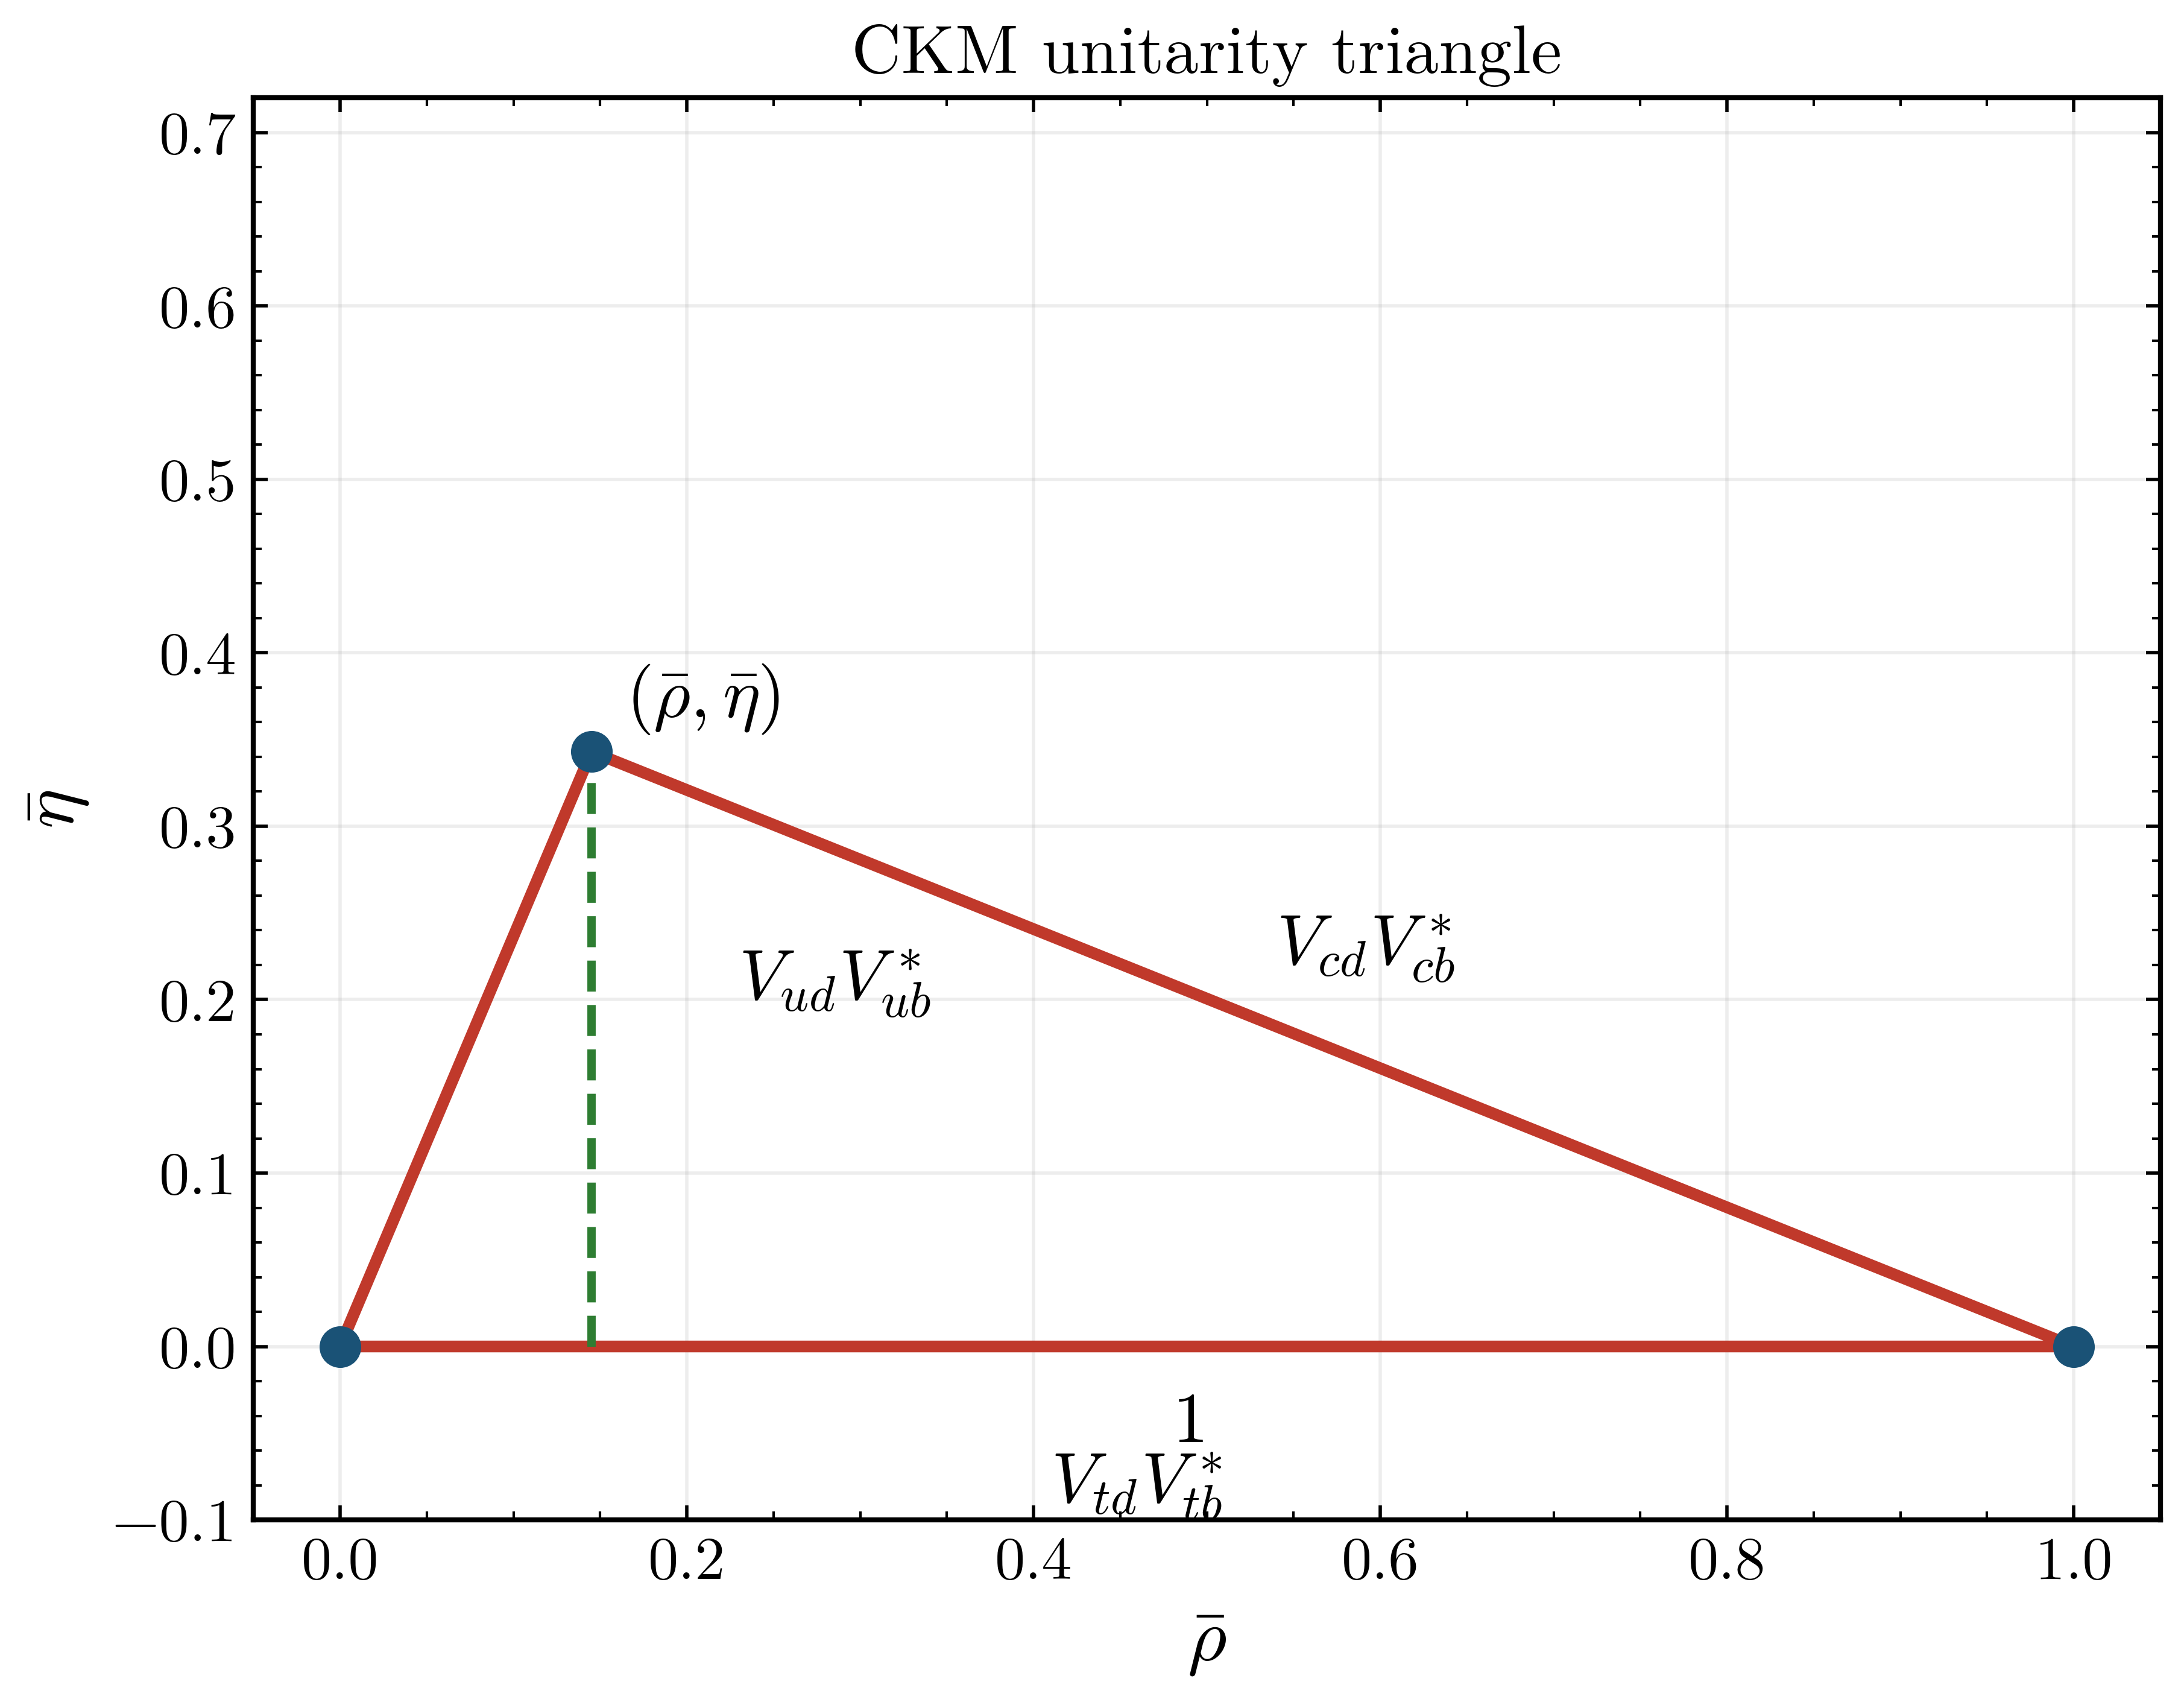
\includegraphics[width=.66\linewidth]{content/FreeElectronQuantumOptics/figures/generated/sm_ckm_unitarity_triangle_dp18.png}
\caption{CKM 幺正性不只是矩阵元素的抽象约束。以 \;\(V_{ud}V_{ub}^*+V_{cd}V_{cb}^*+V_{td}V_{tb}^*=0\) 为例，可把三项画成复平面中的闭合三角形；其非零面积正比于 Jarlskog 不变量；在上下型夸克质量谱均非简并时，它可直接编码夸克扇区的 $CP$ 破坏。图中的顶点取代表性参数点，只用于说明几何结构。}
\label{fig:sm-ckm-unitarity-triangle-dp18}
\end{figure}



最小场内容 \eqnrefs{eq:sm-one-generation-reps-dp11} 不含 $\nu_R$，也不存在维数四的可重整化中微子 Yukawa 项，所以中微子在严格最小可重整化标准模型中无质量，因此也不存在由不同中微子质量本征态相位差产生的真空振荡。现实中的中微子振荡要求扩展场论。只使用标准模型轻场时，最低维的轻子数破坏规范单态是维数五 Weinberg 算符 $(L^T C L)\Phi\Phi/\Lambda$ 的规范收缩；电弱对称性破缺把它转化为 Majorana 中微子质量矩阵，质量基与弱味基的失配由 PMNS 矩阵描述。


% 参数计数已在正文由 $2N_g-1$ 个可消去重相位一行完成；不另设推导框。

\begin{derivation}[从\eqnrefs{eq:ckm-rephasing-dp68}到\eqnrefs{eq:jarlskog-dp11}]
质量本征场仍允许保持质量项不变的矢量式重相位

\begin{equation*}
 u_i\to \ee^{\ii\alpha_i}u_i,
 \qquad
 d_j\to \ee^{\ii\beta_j}d_j.
\end{equation*}
带电流中的 CKM 元素因此变换为
\begin{equation*}
 V_{ij}\to
 \ee^{-\ii\alpha_i}V_{ij}\ee^{\ii\beta_j}.
\end{equation*}
考虑四元积
\begin{equation*}
 X_{ik;jl}\equiv V_{ij}V_{kl}V_{il}^*V_{kj}^*,
 \qquad i\neq k,
 \quad j\neq l.
\end{equation*}
四个因子分别携带相位
\begin{align*}
 V_{ij}:&\quad \ee^{-\ii\alpha_i}\ee^{+\ii\beta_j},\\
 V_{kl}:&\quad \ee^{-\ii\alpha_k}\ee^{+\ii\beta_l},\\
 V_{il}^*:&\quad \ee^{+\ii\alpha_i}\ee^{-\ii\beta_l},\\
 V_{kj}^*:&\quad \ee^{+\ii\alpha_k}\ee^{-\ii\beta_j}.
\end{align*}
相乘后 $\alpha_i,\alpha_k,\beta_j,\beta_l$ 各出现一次正号和一次负号，总相位严格等于 $1$。因此 $X_{ik;jl}$ 以及它的虚部都不依赖质量本征场的重相位选择；单个 CKM 元素的相位则没有这种性质。

取标准三角参数化 $V=R_{23}U_{13}(\delta)R_{12}$。计算\eqnrefs{eq:jarlskog-dp11} 可选择
\begin{equation*}
 J_{\rm CKM}
 =\Im\left(V_{ud}V_{cs}V_{us}^*V_{cd}^*\right).
\end{equation*}
所需四个矩阵元为
\begin{align*}
 V_{ud}&=c_{12}c_{13},\\
 V_{us}&=s_{12}c_{13},\\
 V_{cd}&=-s_{12}c_{23}-c_{12}s_{23}s_{13}\ee^{\ii\delta},\\
 V_{cs}&=c_{12}c_{23}-s_{12}s_{23}s_{13}\ee^{\ii\delta}.
\end{align*}
前两个矩阵元为实数，因此
\begin{align*}
 J_{\rm CKM}
 =c_{12}s_{12}c_{13}^2\,
 \Im\Big[&
 (c_{12}c_{23}-s_{12}s_{23}s_{13}\ee^{\ii\delta})\\
 &\times(-s_{12}c_{23}-c_{12}s_{23}s_{13}\ee^{-\ii\delta})
 \Big].
\end{align*}
把括号展开：
\begin{align*}
 {}&-c_{12}s_{12}c_{23}^2
 -c_{12}^2c_{23}s_{23}s_{13}\ee^{-\ii\delta}\\
 &\qquad
 +s_{12}^2c_{23}s_{23}s_{13}\ee^{\ii\delta}
 +c_{12}s_{12}s_{23}^2s_{13}^2.
\end{align*}
第一项和最后一项为实数；中间两项的虚部为
\begin{align*}
 &c_{12}^2c_{23}s_{23}s_{13}\sin\delta
 +s_{12}^2c_{23}s_{23}s_{13}\sin\delta\\
 &=(c_{12}^2+s_{12}^2)c_{23}s_{23}s_{13}\sin\delta\\
 &=c_{23}s_{23}s_{13}\sin\delta.
\end{align*}
所以
\begin{equation*}
 J_{\rm CKM}
 =c_{12}c_{23}c_{13}^2s_{12}s_{23}s_{13}\sin\delta,
\end{equation*}
即\eqnrefs{eq:jarlskog-dp11}。

三代幺正性进一步固定所有异行异列四元积的相对符号。定义
\begin{equation*}
 \mathcal J_{ij;\alpha\beta}
 \equiv\Im\!\left(
 V_{i\alpha}V_{j\beta}V_{i\beta}^*V_{j\alpha}^*
 \right),
 \qquad i\neq j,\quad \alpha\neq\beta.
\end{equation*}
交换两行或两列都会把括号内的复数变为其复共轭，因此
\begin{equation*}
 \mathcal J_{ji;\alpha\beta}
 =-\mathcal J_{ij;\alpha\beta},
 \qquad
 \mathcal J_{ij;\beta\alpha}
 =-\mathcal J_{ij;\alpha\beta}.
\end{equation*}
再固定一对不同的行 $i,j$ 与一列 $\alpha$。行正交性给
\begin{equation*}
 \sum_{\lambda=1}^{3}V_{i\lambda}V_{j\lambda}^*=0.
\end{equation*}
乘以 $V_{i\alpha}^*V_{j\alpha}$ 并取虚部，$\lambda=\alpha$ 项为实数，于是其余两列 $\beta,\gamma$ 满足
\begin{equation*}
 \mathcal J_{ij;\beta\alpha}
 +\mathcal J_{ij;\gamma\alpha}=0.
\end{equation*}
结合列交换的反对称性，固定行对时三个不同列对的四元积虚部具有相同绝对值，并按列指标的奇偶排列改变符号。

为了比较不同的行对，固定两列 $\alpha\neq\beta$ 与一行 $i$。列正交性给
\begin{equation*}
 \sum_{r=1}^{3}V_{r\alpha}V_{r\beta}^*=0.
\end{equation*}
乘以 $V_{i\alpha}^*V_{i\beta}$ 并取虚部，$r=i$ 项为
$|V_{i\alpha}|^2|V_{i\beta}|^2$，其虚部为零，因此剩余两行 $j,k$ 满足
\begin{equation*}
 \Im\!\left(
 V_{j\alpha}V_{j\beta}^*
 V_{i\alpha}^*V_{i\beta}
 \right)
 +
 \Im\!\left(
 V_{k\alpha}V_{k\beta}^*
 V_{i\alpha}^*V_{i\beta}
 \right)=0.
\end{equation*}
把每一项重新排列成 $\mathcal J$ 的定义，并使用行交换的反对称性，就得到固定列对时不同的行对具有相同绝对值，并按行指标排列改变符号。以
\begin{equation*}
 \mathcal J_{12;12}
 =\Im(V_{ud}V_{cs}V_{us}^*V_{cd}^*)
 \equiv J_{\rm CKM}
\end{equation*}
固定总体符号，便得到三代幺正矩阵的恒等式
\begin{equation*}
 \mathcal J_{ij;\alpha\beta}
 =J_{\rm CKM}\,\epsilon_{ijk}\epsilon_{\alpha\beta\gamma},
\end{equation*}
其中 $k$ 与 $\gamma$ 分别是剩余的第三个行、列指标。这就是三代幺正矩阵的一般四元积恒等式。

\end{derivation}

\begin{derivation}[从\eqnrefs{eq:jarlskog-dp11}到\eqnrefs{eq:jarlskog-determinant-dp11}]
定义两个厄米矩阵

\begin{equation*}
 H_u\equiv Y_uY_u^\dagger,
 \qquad
 H_d\equiv Y_dY_d^\dagger.
\end{equation*}
在共同左手弱基变换 $Q_L\to U_QQ_L$ 下，
\begin{equation*}
 H_u\to U_QH_uU_Q^\dagger,
 \qquad
 H_d\to U_QH_dU_Q^\dagger.
\end{equation*}
因此对易子
\begin{equation*}
 C\equiv[H_u,H_d]
\end{equation*}
只作相似变换 $C\to U_QCU_Q^\dagger$，所以 $\det C$ 与弱基选择无关。又因为 $H_u,H_d$ 厄米，
\begin{equation*}
 C^\dagger=-C,
\end{equation*}
三代时 $\det C$ 必为纯虚数。

选择上型夸克质量基，并简记
\begin{equation*}
 a_i\equiv y_{u_i}^2,
 \qquad
 b_\alpha\equiv y_{d_\alpha}^2.
\end{equation*}
于是
\begin{equation*}
 H_u=\operatorname{diag}(a_1,a_2,a_3),
 \qquad
 H_d=V\operatorname{diag}(b_1,b_2,b_3)V^\dagger,
\end{equation*}
其中 $V=V_{\rm CKM}$。对易子的矩阵元为
\begin{align*}
 C_{ij}
 &=(a_i-a_j)(H_d)_{ij},\\
 (H_d)_{ij}
 &=\sum_{\alpha=1}^{3}V_{i\alpha}b_\alpha V_{j\alpha}^*.
\end{align*}
特别地 $C_{ii}=0$。因此三阶行列式只剩两个三循环项：
\begin{equation*}
 \det C=C_{12}C_{23}C_{31}+C_{13}C_{21}C_{32}.
\end{equation*}
定义
\begin{equation*}
 \Delta_u\equiv
 (a_1-a_2)(a_1-a_3)(a_2-a_3).
\end{equation*}
第一个循环的上型谱因子为
\begin{align*}
 &(a_1-a_2)(a_2-a_3)(a_3-a_1)\\
 &=-\Delta_u,
\end{align*}
第二个循环的上型谱因子为
\begin{align*}
 &(a_1-a_3)(a_2-a_1)(a_3-a_2)\\
 &=+\Delta_u.
\end{align*}
又因为 $H_d$ 厄米，令
\begin{equation*}
 z\equiv(H_d)_{12}(H_d)_{23}(H_d)_{31},
\end{equation*}
则
\begin{equation*}
 (H_d)_{13}(H_d)_{21}(H_d)_{32}=z^*.
\end{equation*}
所以
\begin{align*}
 \det C
 &=\Delta_u(z^*-z)\\
 &=-2\ii\Delta_u\Im z.
\end{align*}
问题于是化为计算 $\Im z$。

由于单位矩阵的非对角元为零，给 $H_d$ 加上任意常数倍单位矩阵都不改变 $z$。因此可以从所有 $b_\alpha$ 中减去 $b_3$，定义
\begin{equation*}
 x\equiv b_1-b_3,
 \qquad
 y\equiv b_2-b_3.
\end{equation*}
对 $i\neq j$，
\begin{equation*}
 (H_d)_{ij}
 =xV_{i1}V_{j1}^*+yV_{i2}V_{j2}^*.
\end{equation*}
于是 $z$ 是 $x,y$ 的三次齐次多项式。纯 $x^3$ 项为
\begin{equation*}
 x^3|V_{11}V_{21}V_{31}|^2,
\end{equation*}
纯 $y^3$ 项为
\begin{equation*}
 y^3|V_{12}V_{22}V_{32}|^2,
\end{equation*}
二者都为实数，不贡献 $\Im z$。

$x^2y$ 的三个交叉项的虚部分别是
\begin{align*}
 \Im\!\big[(V_{11}V_{21}^*)(V_{21}V_{31}^*)(V_{32}V_{12}^*)\big]
 &=-J_{\rm CKM}|V_{21}|^2,\\
 \Im\!\big[(V_{11}V_{21}^*)(V_{22}V_{32}^*)(V_{31}V_{11}^*)\big]
 &=-J_{\rm CKM}|V_{11}|^2,\\
 \Im\!\big[(V_{12}V_{22}^*)(V_{21}V_{31}^*)(V_{31}V_{11}^*)\big]
 &=-J_{\rm CKM}|V_{31}|^2.
\end{align*}
三代幺正矩阵的四元积满足
\begin{equation*}
 \Im(V_{i\alpha}V_{j\beta}V_{i\beta}^*V_{j\alpha}^*)
 =J_{\rm CKM}\,\epsilon_{ijk}\epsilon_{\alpha\beta\gamma},
\end{equation*}
其中未写出的 $k,\gamma$ 是各自剩余的第三个指标。由第一列归一化
\begin{equation*}
 |V_{11}|^2+|V_{21}|^2+|V_{31}|^2=1,
\end{equation*}
故全部 $x^2y$ 项的虚部为
\begin{equation*}
 -J_{\rm CKM}x^2y.
\end{equation*}
对 $xy^2$ 项逐个应用四元积恒等式，三个虚部分别是
\begin{align*}
 \Im(V_{11}V_{22}V_{12}^*V_{21}^*)|V_{32}|^2
 &=+J_{\rm CKM}|V_{32}|^2,\\
 \Im(V_{21}V_{32}V_{22}^*V_{31}^*)|V_{12}|^2
 &=+J_{\rm CKM}|V_{12}|^2,\\
 \Im(V_{31}V_{12}V_{32}^*V_{11}^*)|V_{22}|^2
 &=+J_{\rm CKM}|V_{22}|^2.
\end{align*}
三项相加后利用第二列归一化得到
\begin{equation*}
 +J_{\rm CKM}xy^2.
\end{equation*}
因此
\begin{align*}
 \Im z
 &=J_{\rm CKM}xy(y-x)\\
 &=-J_{\rm CKM}(b_1-b_2)(b_1-b_3)(b_2-b_3)\\
 &=-J_{\rm CKM}\Delta_d.
\end{align*}
代回 $\det C=-2\ii\Delta_u\Im z$：
\begin{equation*}
 \det[H_u,H_d]
 =2\ii J_{\rm CKM}\Delta_u\Delta_d,
\end{equation*}
即\eqnrefs{eq:jarlskog-determinant-dp11}。

这个推导还直接给出两个退化检查：若任意两种上型 Yukawa 本征值相同，则 $\Delta_u=0$；若任意两种下型本征值相同，则 $\Delta_d=0$。任一情形都使所有弱基不变的 $CP$ 奇量消失，因为相应简并子空间内出现额外的味旋转自由度。
\end{derivation}


% 幺正三角形面积由复平面二维行列式一行得到，正文已给出结果；不另设推导框。


\subsection{GIM 抵消与环级味改变中性流}\label{subsec:sm-gim-dp83}

质量本征基中的光子、胶子和 $Z$ 中性流都与味指标成正比于单位矩阵，因此树级中性流不会把一个下型夸克质量本征态变成另一个。两个带电弱顶角却可以在圈内先把外部 $d_j$ 变成上型夸克 $u_i$，再变回 $d_k$；味改变中性流因此第一次在圈级出现。每个单独圈图一般依赖规范和中间参数化，只有把给定过程在该阶所需的规范不变图集合相加以后，才能把内部质量依赖压缩成物理圈函数。

对一般 $d_j\to d_k$（$j\ne k$）的一圈味改变中性流，先选取一组完备、线性无关的外部 Lorentz--Dirac 算符结构 $\mathcal K_a(p_{\rm ext})$。把给定微扰阶所需的顶角图、自能图、Goldstone 与鬼场图按规范不变组合求和后，振幅可唯一分解为
\begin{equation}
 \boxed{
 \mathcal A_{j\to k}^{\rm FCNC}
 =\sum_a \mathcal K_a(p_{\rm ext})\,C_a^{jk},
 \qquad
 C_a^{jk}
 =\sum_iV_{ik}^*V_{ij}F_a(x_i),}
 \label{eq:sm-gim-loop-sum-dp83}
\end{equation}
其中
\begin{equation*}
 x_i\equiv\frac{m_{u_i}^2}{m_W^2},
 \qquad u_i\in\{u,c,t\}.
\end{equation*}
$F_a(x_i)$ 是第 $a$ 个独立算符系数在内部上型夸克质量为 $m_{u_i}$ 时的完整一圈函数；所有与内部味无关的规范耦合、外部运动学与归一化因子都已按同一方式包含在 $\mathcal K_a$ 或 $F_a$ 的定义中。两个带电流顶角分别给出 $V_{ij}$ 与 $V_{ik}^*$，因此内部味只通过 $V_{ik}^*V_{ij}$ 与 $x_i$ 进入。

CKM 幺正性给出非对角关系
\begin{equation}
 \boxed{
 \sum_iV_{ik}^*V_{ij}=(V^\dagger V)_{kj}=0,
 \qquad j\ne k.}
 \label{eq:sm-gim-unitarity-dp83}
\end{equation}
于是对每一个独立算符系数、对任意参考点 $x_*$ 都有恒等式
\begin{equation}
 \boxed{
 C_a^{jk}
 =\sum_iV_{ik}^*V_{ij}\,[F_a(x_i)-F_a(x_*)],
 \qquad j\ne k.}
 \label{eq:sm-gim-subtracted-exact-dp85}
\end{equation}
若所有内部上型夸克质量简并，则所有 $x_i$ 相同，右端逐项差值相同并被\eqnrefs{eq:sm-gim-unitarity-dp83} 消去，因此每个 $C_a^{jk}$ 都为零。这就是 GIM 机制与具体过程无关的代数核心。

只有在所考察的 $F_a(x)$ 在 $x=0$ 邻域至少二次可微、并且参与展开的全部 $x_i\ll1$ 时，才把\eqnrefs{eq:sm-gim-subtracted-exact-dp85} 进一步展开。取 $x_*=0$，Taylor 定理给
\begin{equation}
 \boxed{
 C_a^{jk}
 =F_a'(0)
 \sum_iV_{ik}^*V_{ij}\frac{m_{u_i}^2}{m_W^2}
 +\mathcal R_{a,jk}^{(\ge2)},}
 \label{eq:sm-gim-mass-suppression-dp83}
\end{equation}
其中 $\mathcal R_{a,jk}^{(\ge2)}$ 从 $x_i^2$ 阶开始，节末推导给出显式余项界。若具体圈函数含 $x\ln x$ 等非解析小质量项，或顶夸克满足 $x_t=O(1)$，则直接使用\eqnrefs{eq:sm-gim-subtracted-exact-dp85} 的精确差值，不使用局域 Taylor 形式。

\begin{derivation}[从\eqnrefs{eq:sm-gim-loop-sum-dp83}到\eqnrefs{eq:sm-gim-mass-suppression-dp83}]
质量本征基中的夸克带电流为
\begin{equation*}
 \Lag_{\rm CC}^{q}
 =-\frac{\hbar c\,g}{\sqrt2}
 \left[
 \bar u_i\gamma^\mu P_LV_{ij}d_j\,\mathcal W_\mu^+
 +\bar d_j\gamma^\mu P_LV_{ij}^*u_i\,\mathcal W_\mu^-
 \right].
\end{equation*}
考虑 $d_j\to d_k$、$j\neq k$ 的一圈味改变中性流。Dyson 展开中任意包含两个带电流顶角的收缩，都含味因子
\begin{equation*}
 V_{ij}V_{ik}^*=V_{ik}^*V_{ij},
\end{equation*}
因为第一个顶角把外部 $d_j$ 连接到内部 $u_i$，第二个厄米共轭顶角再把同一内部味 $u_i$ 连接到外部 $d_k$。

给定外部粒子与动量后，选一组完备、线性无关的 Lorentz--Dirac 算符基 $\{\mathcal K_a(p_{\rm ext})\}$。同一微扰阶的全部规范完成图求和后，任意内部味 $i$ 的贡献都能按这组基展开：
\begin{equation*}
 \mathcal A_{j\to k}^{(i)}
 =V_{ik}^*V_{ij}
 \sum_a\mathcal K_a(p_{\rm ext})F_a(x_i),
 \qquad
 x_i=\frac{m_{u_i}^2}{m_W^2}.
\end{equation*}
这里 $F_a$ 由实际圈积分定义。例如在维数正规化中，每个 $F_a$ 都来自形如
\begin{equation*}
 \mu_{\rm DR}^{2\epsilon}
 \int\frac{\dd^d\ell}{(2\pi)^d}
 \frac{N_a(\ell,p_{\rm ext};m_{u_i},m_W)}
 {\prod_r D_r(\ell,p_{\rm ext};m_{u_i},m_W)}
\end{equation*}
的积分及同阶规范完成项。对内部味求和并交换有限求和与算符基展开，得到
\begin{align*}
 \mathcal A_{j\to k}^{\rm FCNC}
 &=\sum_i\mathcal A_{j\to k}^{(i)}\\
 &=\sum_a\mathcal K_a(p_{\rm ext})
 \left[\sum_iV_{ik}^*V_{ij}F_a(x_i)\right].
\end{align*}
因此
\begin{equation*}
 C_a^{jk}=\sum_iV_{ik}^*V_{ij}F_a(x_i),
\end{equation*}
即正文\eqnrefs{eq:sm-gim-loop-sum-dp83}。

CKM 幺正性 $V^\dagger V=I$ 的非对角元满足
\begin{equation*}
 \sum_iV_{ik}^*V_{ij}=0,
 \qquad j\neq k.
\end{equation*}
对任意参考点 $x_*$，逐个算符系数加减同一个 $F_a(x_*)$：
\begin{align*}
 C_a^{jk}
 &=\sum_iV_{ik}^*V_{ij}
 \left[F_a(x_i)-F_a(x_*)+F_a(x_*)\right]\\
 &=\sum_iV_{ik}^*V_{ij}[F_a(x_i)-F_a(x_*)]
 +F_a(x_*)\sum_iV_{ik}^*V_{ij}\\
 &=\sum_iV_{ik}^*V_{ij}[F_a(x_i)-F_a(x_*)].
\end{align*}
这就是\eqnrefs{eq:sm-gim-subtracted-exact-dp85}。若 $x_i=x_*$ 对所有内部味都成立，则每个独立算符系数 $C_a^{jk}$ 都等于零，因而完整振幅为零。

若 $F_a$ 在连接 $x_*$ 与 $x_i$ 的区间可微，微积分基本定理还给出精确质量差表示
\begin{align*}
 F_a(x_i)-F_a(x_*)
 &=\int_{x_*}^{x_i}\dd y\,F_a'(y)\\
 &=(x_i-x_*)\int_0^1\dd t\,
 F_a'\!\left[x_*+t(x_i-x_*)\right],
\end{align*}
因此
\begin{equation*}
 C_a^{jk}
 =\sum_iV_{ik}^*V_{ij}(x_i-x_*)
 \int_0^1\dd t\,
 F_a'\!\left[x_*+t(x_i-x_*)\right].
\end{equation*}
这条等式直接表明共同的内部质量部分被消去，剩余量由质量劈裂加权。

对轻内部质量取 $x_*=0$。若 $F_a\in C^3([0,x_{\max}])$，Taylor 定理带积分余项给
\begin{equation*}
 F_a(x_i)
 =F_a(0)+x_iF_a'(0)+\frac{x_i^2}{2}F_a''(0)
 +\frac{x_i^3}{2}\int_0^1\dd t\,(1-t)^2F_a^{(3)}(tx_i).
\end{equation*}
代入并使用 $\sum_iV_{ik}^*V_{ij}=0$：
\begin{equation*}
 C_a^{jk}
 =F_a'(0)\sum_iV_{ik}^*V_{ij}x_i
 +\mathcal R_{a,jk}^{(\ge2)},
\end{equation*}
其中
\begin{align*}
 \mathcal R_{a,jk}^{(\ge2)}
 &\equiv
 \frac{F_a''(0)}2
 \sum_iV_{ik}^*V_{ij}x_i^2+R_{a,jk}^{(3)},\\
 R_{a,jk}^{(3)}
 &\equiv
 \frac12\sum_iV_{ik}^*V_{ij}x_i^3
 \int_0^1\dd t\,(1-t)^2F_a^{(3)}(tx_i).
\end{align*}
于是
\begin{align*}
 |R_{a,jk}^{(3)}|
 &\le\frac16
 \max_{0\le y\le x_{\max}}|F_a^{(3)}(y)|
 \sum_i|V_{ik}^*V_{ij}|x_i^3,\\
 |\mathcal R_{a,jk}^{(\ge2)}|
 &\le\frac{|F_a''(0)|}{2}
 \sum_i|V_{ik}^*V_{ij}|x_i^2
 +|R_{a,jk}^{(3)}|.
\end{align*}
最后用 $x_i=m_{u_i}^2/m_W^2$ 即得到正文\eqnrefs{eq:sm-gim-mass-suppression-dp83} 及其余项控制。若 $F_a$ 在零点附近非解析，或某个 $x_i$ 不小，则保留精确差值\eqnrefs{eq:sm-gim-subtracted-exact-dp85}。
\end{derivation}


\subsection{量子规范一致性、全局流与拓扑}\label{subsec:sm-gauge-anomaly-cancellation-dp32}

经典作用量把同一规范轨道上的场配置识别为同一物理态。量子化后的物理态空间必须保持这种规范等价：若圈修正让规范等价的场配置得到不同的量子振幅，纵向的非物理自由度就不能再从可观测振幅中一致消去，理论本身会失去幺正的物理态解释。手征费米子恰好会带来这种风险，因为定义费米子路径积分测度时所需的紫外正则化可能产生一个非平凡 Jacobian。这个由量子测度破坏经典规范冗余的现象称为规范反常。

是否发生这种破坏，可以直接由三角图中的群表示因子判断。对三个非阿贝尔规范流，其系数由对称迹
\begin{equation*}
 d_R^{abc}=2\Tr_R\!\left[T^a\{T^b,T^c\}\right]
\end{equation*}
控制。若被破坏的是局域规范流，这个系数必须在完整的左手 Weyl 费米子谱上精确相消，而不能把反常解释成可接受的量子修正。

对一般左手 Weyl 场 $f$，若其表示为 $R_{3f}\otimes R_{2f}$、超荷为 $Y_f$，先把三个群论数字定义清楚。$d_a(R)$ 是表示空间维数；Dynkin 指标 $T_a(R)$ 由
\begin{equation*}
 \Tr_R(T^AT^B)=T_a(R)\delta^{AB}
\end{equation*}
定义，因而控制两个非阿贝尔生成元进入三角图时的迹；$SU(3)$ 三次反常指标 $A_3(R)$ 则由对称三生成元迹相对于基本表示的系数定义，共轭表示满足 $A_3(\bar R)=-A_3(R)$。因此，混合反常使用 $T_a(R)$，纯 $SU(3)^3$ 反常使用对三生成元共轭敏感的 $A_3(R)$。四维标准模型相关的局域规范反常系数可统一写成
\begin{equation}
\boxed{
\begin{aligned}
C_{333}&=\sum_f d_2(R_{2f})A_3(R_{3f}),\\
C_{33Y}&=\sum_f d_2(R_{2f})Y_fT_3(R_{3f}),\\
C_{22Y}&=\sum_f d_3(R_{3f})Y_fT_2(R_{2f}),\\
C_{YYY}&=\sum_f d_3(R_{3f})d_2(R_{2f})Y_f^3,\\
C_{{\rm grav}^2Y}&=\sum_f d_3(R_{3f})d_2(R_{2f})Y_f.
\end{aligned}}
\label{eq:general-chiral-anomaly-coefficients-dp75}
\end{equation}
局域量子规范一致性要求这些系数全部为零。$SU(2)$ 的有限维表示为实或伪实，因此没有独立的局域 $SU(2)^3$ 三次反常；但局域三角图并未穷尽全局拓扑障碍。

统一采用左手 Weyl 场记账最为直接。右手场 $\psi_R$ 改写为左手荷共轭场 $\psi_R^c$ 后，非阿贝尔表示变为共轭表示，$U(1)$ 荷变号。标准模型每一代的左手场谱为
\begin{align}
 Q_L&:(\mathbf3,\mathbf2,+\tfrac16),&
 u_R^c&:(\bar{\mathbf3},\mathbf1,-\tfrac23),\\
 d_R^c&:(\bar{\mathbf3},\mathbf1,+\tfrac13),&
 L_L&:(\mathbf1,\mathbf2,-\tfrac12),\\
 e_R^c&:(\mathbf1,\mathbf1,+1).
 \label{eq:sm-left-weyl-anomaly-set-dp11}
\end{align}
这里三元组依次表示 $SU(3)_c$、$SU(2)_L$ 表示与超荷 $Y$。这一场谱必须同时满足
\begin{equation}
 \boxed{
 C_{333}^{\rm anom}=
 C_{33Y}^{\rm anom}=
 C_{22Y}^{\rm anom}=
 C_{YYY}^{\rm anom}=
 C_{{\rm grav}^2Y}^{\rm anom}=0.}
 \label{eq:sm-gauge-anomaly-cancellation-dp32}
\end{equation}
此外，纯 $[SU(3)_c]^3$ 反常也必须抵消。$SU(2)$ 基本表示是伪实表示，因此局部三角图不会产生 $SU(2)^3$ 反常，但局部微扰展开并未检查规范变换空间的全局拓扑。把欧几里得四维时空在无穷远固定后紧化为 $S^4$，一个大规范变换可看成连续映射 $U:S^4\to SU(2)$。记号 $\pi_4(SU(2))$ 表示这类映射在连续变形下的同伦分类；$\pi_4(SU(2))=\mathbb Z_2$ 意味着只有平凡类与一个不能连续缩回恒等变换的非平凡类。Witten 的全局反常定理指出：沿这个非平凡类作规范变换时，单个左手 $SU(2)$ 基本二重态的费米子泛函积分整体变号。因此含 $N_D$ 个基本左手二重态时总符号为 $(-1)^{N_D}$，量子规范不变性要求 $N_D$ 为偶数。标准模型每一代含三个颜色副本的 $Q_L$ 与一个 $L_L$，故 $N_D=4$，模二全局障碍消失。

规范不变的 Yukawa 耦合还把左、右手超荷彼此联系。若暂以
\begin{equation*}
 Y_Q=q,\quad Y_u=u,\quad Y_d=d,\quad
 Y_L=\ell,\quad Y_e=e,\quad Y_\Phi=h
\end{equation*}
表示一代超荷，则三条 Yukawa 单态条件与两个独立的线性反常条件可整理成
\begin{equation}
\boxed{
 u=q+h,\qquad d=q-h,\qquad e=\ell-h,\qquad
 3q+\ell=0,\qquad
 6q-3u-3d+2\ell-e=0.}
\label{eq:sm-hypercharge-constraint-system-dp68}
\end{equation}
这组方程把相对超荷固定到一个整体归一化。取 Higgs 约定 $h=1/2$ 后得到
\begin{equation}
 \boxed{
 Y_Q=\frac16,\quad Y_u=\frac23,\quad Y_d=-\frac13,\quad
 Y_L=-\frac12,\quad Y_e=-1,\quad Y_\Phi=\frac12.}
 \label{eq:sm-hypercharge-solution-dp32}
\end{equation}
因此标准模型超荷并不是只为重现实验电荷而填写的一张表；同一组数还必须允许 Yukawa 质量耦合，并同时满足局域与全局规范一致性条件。任何改变手征费米子场内容的新物理模型，都必须重新检查这些条件。

\label{subsec:sm-global-axial-anomaly-dp32}
局域规范反常的精确抵消保证量子规范理论可以一致定义；与此不同，物理全局流允许出现由量子测度产生的反常，并留下可观测的拓扑效应。

规范反常必须抵消，但全局流的反常可以成为真实的量子效应。对一个 Dirac 费米子，经典轴流
\begin{equation*}
 J_5^\mu=\bar\psi\gamma^\mu\gamma^5\psi
\end{equation*}
在有质量时已经满足 $\partial_\mu J_5^\mu=(2\ii mc/\hbar)\bar\psi\gamma^5\psi$；量子化后，费米子测度还产生规范场的拓扑密度。对单位电荷 QED 费米子，采用对偶场强的定义后，结果为
\begin{equation}
 \boxed{
 \partial_\mu J_5^\mu
 =\frac{2\ii mc}{\hbar}\bar\psi\gamma^5\psi
 +\frac{g_{\rm em}^2}{8\pi^2}
 F_{\mu\nu}^{\rm geo}{}^\star\!F_{\rm geo}^{\mu\nu}
 =\frac{2\ii mc}{\hbar}\bar\psi\gamma^5\psi
 +\frac{e^2}{8\pi^2\hbar^2}
 F_{\mu\nu}{}^\star\!F^{\mu\nu}.}
 \label{eq:abj-anomaly-qed-dp11}
\end{equation}
第二个等号使用 \eqnrefs{eq:sm-photon-geo-si-bridge-dp75}，其中末项的 $F_{\mu\nu}$ 是前面 QED 章节固定的 SI 电磁场强。这里异常的是全局轴对称性，而不是电磁 $U(1)$ 规范对称性；矢量规范流仍必须保持守恒。

在路径积分量子化中，费米子场不是对每个时空点上的普通数值直接积分，而是先在一组完备正交的单粒子函数 $\{\phi_n(x)\}$ 上展开。若
\begin{equation*}
 q(x)=\sum_n a_n\phi_n(x),
 \qquad
 \bar q(x)=\sum_n\bar b_n\phi_n^\dagger(x),
\end{equation*}
则 $a_n,\bar b_n$ 是反交换的 Grassmann 系数。所谓\emph{费米子路径积分测度}，就是对全部这些系数作 Berezin 积分的乘积
\begin{equation*}
 \mathcal Dq\,\mathcal D\bar q
 \equiv\prod_n\dd a_n\,\dd\bar b_n.
\end{equation*}
场的局域线性变换会同时线性变换无穷多个系数，因此测度一般获得一个 Jacobian。Fujikawa 方法的核心就是用保持规范协变性的正则化来计算这个无穷维 Jacobian；若 Jacobian 不等于一，经典作用量的对称性在量子理论中便产生反常。

对 $N_f$ 个 QCD 基本表示夸克，考虑共同的轴向旋转
\begin{equation}
\boxed{
 q_f\to \ee^{\ii\alpha\gamma^5}q_f,
 \qquad
 \bar q_f\to \bar q_f\ee^{\ii\alpha\gamma^5}.}
\label{eq:qcd-singlet-axial-rotation-dp68}
\end{equation}
经典无质量作用量在这一变换下不变，但路径积分测度的 Jacobian 不为一。因此味单态轴流 $J_5^\mu=\sum_f\bar q_f\gamma^\mu\gamma^5q_f$ 满足
\begin{equation}
 \boxed{
 \partial_\mu J_5^\mu
 =\sum_f\frac{2\ii m_fc}{\hbar}\bar q_f\gamma^5q_f
 +\frac{N_f g_s^2}{16\pi^2}
 \mathcal F_{\mu\nu}^a{}^\star\!\mathcal F^{a\mu\nu}.}
 \label{eq:qcd-singlet-axial-anomaly-dp32}
\end{equation}
所以轻夸克极限中的 $U(1)_A$ 不会像非单态 $SU(N_f)_A$ 那样产生额外的轻 Goldstone 模式；非微扰 QCD 的手征凝聚与轴反常分别控制非单态和味单态两个不同的对称性问题。

电弱 $SU(2)_L$ 的拓扑扇区还使经典重整化标准模型中的重子数 $B$ 与轻子数 $L$ 发生全局反常。拓扑荷定义为
\begin{equation}
\boxed{
 \nu=\frac{g^2}{32\pi^2}
 \int\dd^4 x\,
 \mathcal W_{\mu\nu}^I{}^\star\!\mathcal W^{I\mu\nu}
 \in\mathbb Z.}
\label{eq:electroweak-topological-charge-dp68}
\end{equation}
这里的\emph{零模}是欧几里得手征 Dirac 算符满足 $\slashed D_E\psi_0=0$ 的归一化本征函数。Atiyah--Singer 指数定理给出表示 $R$ 中左右手零模数之差
\begin{equation*}
 n_L-n_R=2T(R)\nu.
\end{equation*}
对 $SU(2)$ 基本表示 $T(\mathbf2)=1/2$，所以 $|\nu|=1$ 的拓扑背景为每个左手弱二重态提供一个不可由非零本征值配对消去的手征零模。Grassmann 路径积分只有在外场插入把这些零模全部饱和时才非零；由这些零模诱导的局域多费米子结构称为 't Hooft 顶点。每一代的三个颜色 $Q_L$ 二重态和一个 $L_L$ 二重态因而共同给出一组 $QQQL$ 型插入。对一般世代数 $N_g$，相应选择定则为
\begin{equation}
 \boxed{
 \Delta B=\Delta L=N_g\nu,\qquad
 \Delta(B-L)=0,\qquad
 \Delta(B+L)=2N_g\nu.}
 \label{eq:sm-bplusl-selection-dp32}
\end{equation}
这与规范反常抵消并不矛盾：$B,L$ 是物理全局流，而规范反常决定局域规范冗余能否在量子理论中一致实现。加入维数五轻子数破坏相互作用后，轻子数还会出现独立的显式 $\Delta L=2$ 破缺，因此拓扑反常与高维算符破缺必须分别处理。

QCD 还允许一个不改变局域规范对称性的拓扑项。采用前述场强与对偶张量约定，把它定义为
\begin{equation}
 \boxed{
 \frac{S_{\theta}}{\hbar}
 =\theta_s\frac{g_s^2}{32\pi^2}
 \int\dd^4x\,
 \mathcal F_{\mu\nu}^a{}^\star\!\mathcal F^{a\mu\nu},}
 \label{eq:qcd-theta-action-dp89}
\end{equation}
其中 $\theta_s$ 是无量纲 QCD 拓扑角。味空间的轴向重相位会同时平移 $\theta_s$ 并改变夸克质量矩阵的整体复相位；这两种变化不是两个独立物理效应。真正与夸克场基底选择无关的强 CP 参数是
\begin{equation}
 \boxed{
 \bar\theta=\theta_s+\arg\det(M_uM_d).}
 \label{eq:strong-cp-theta-bar-dp11}
\end{equation}
若存在一个严格无质量的夸克，就可以用其轴向重相位消去 $\bar\theta$；真实夸克质量均非零后，这个自由度消失，而实验又要求 $|\bar\theta|$ 极小，由此形成强 CP 问题。这个参数与 CKM 相位、微扰 QCD 的 $\beta$ 函数和电弱 $B+L$ 选择定则都不是同一个物理量。

局域规范反常是量子一致性障碍，必须在完整手征物质谱上抵消；Witten 的 $SU(2)$ 全局反常是规范场配置空间的拓扑一致性条件，同样必须消失；轴流、$B$ 和 $L$ 这类物理全局流则可以具有非零反常，并留下 $\pi^0\to\gamma\gamma$、$U(1)_A$ 质量结构、电弱 $B+L$ 选择定则和强 CP 等可观测后果。三者都与量子测度有关，但逻辑地位不同。


\begin{derivation}[从\eqnrefs{eq:sm-left-weyl-anomaly-set-dp11}到\eqnrefs{eq:sm-gauge-anomaly-cancellation-dp32}]
先说明为什么规范反常只需要检查正文列出的那些群论迹。对一个左手 Weyl 费米子，三个外部规范玻色子与费米子环相连时，两种相反顶角次序的群因子分别为
\begin{equation*}
 \Tr_R(T^aT^bT^c),
 \qquad
 \Tr_R(T^aT^cT^b).
\end{equation*}
三角图的宇称奇部分在交换后两个外腿时是对称的，因此两种次序相加后只保留
\begin{equation*}
 \Tr_R\!\left[T^a\{T^b,T^c\}\right]
 =\frac12d_R^{abc}.
\end{equation*}
动量积分与正则化决定共同的数值前因子，而一个给定费米子谱是否无规范反常只取决于全部左手 Weyl 场的这些群因子之和是否为零。若其中一个或多个外腿属于 $U(1)_Y$，相应生成元就是超荷乘单位矩阵，于是四类局域反常系数分别化为
\begin{align*}
 [SU(N)]^2U(1)_Y &: \sum_f Y_fT(R_f),\\
 [U(1)_Y]^3 &: \sum_f d(R_f)Y_f^3,\\
 {\rm grav}^2U(1)_Y &: \sum_f d(R_f)Y_f,\\
 [SU(N)]^3 &: \sum_f d_{R_f}^{abc}.
\end{align*}
这里 $d(R_f)$ 表示其余内部指标的多重度。规范理论要求这些群论系数在全部左手 Weyl 场上求和后同时为零。

现在把一代标准模型全部改写成左手 Weyl 场
\begin{equation*}
 Q_L:(\mathbf3,\mathbf2)_{1/6},\quad
 u_R^c:(\bar{\mathbf3},\mathbf1)_{-2/3},\quad
 d_R^c:(\bar{\mathbf3},\mathbf1)_{1/3},\quad
 L_L:(\mathbf1,\mathbf2)_{-1/2},\quad
 e_R^c:(\mathbf1,\mathbf1)_{1}.
\end{equation*}
把共同的三角圈动量积分和规范耦合常数提出以后，定义纯群论反常系数
\begin{align*}
 \mathfrak A_{33Y}
 &\equiv\sum_{\text{左手 Weyl }f}d_2(f)Y_fT_3(R_f),\\
 \mathfrak A_{22Y}
 &\equiv\sum_f d_3(f)Y_fT_2(R_f),\\
 \mathfrak A_{YYY}
 &\equiv\sum_f d_3(f)d_2(f)Y_f^3,\\
 \mathfrak A_{{\rm grav}^2Y}
 &\equiv\sum_f d_3(f)d_2(f)Y_f.
\end{align*}
其中 $d_3,d_2$ 分别是颜色和弱表示维数。利用 $T(\mathbf3)=T(\bar{\mathbf3})=T(\mathbf2)=1/2$，一代标准模型逐项给
\begin{align*}
 \mathfrak A_{33Y}
 &=2\!\left(\frac16\right)\frac12
 +\left(-\frac23\right)\frac12
 +\left(\frac13\right)\frac12=0,\\
 \mathfrak A_{22Y}
 &=3\!\left(\frac16\right)\frac12
 +\left(-\frac12\right)\frac12=0,\\
 \mathfrak A_{YYY}
 &=6\left(\frac16\right)^3
 +3\left(-\frac23\right)^3
 +3\left(\frac13\right)^3
 +2\left(-\frac12\right)^3+1^3=0,\\
 \mathfrak A_{{\rm grav}^2Y}
 &=6\left(\frac16\right)
 +3\left(-\frac23\right)
 +3\left(\frac13\right)
 +2\left(-\frac12\right)+1=0.
\end{align*}
这些等式就是四类反常的群论系数本身为零，而不是只说明它们“与某个零表达式成正比”。
对 $[SU(3)_c]^3$，基本表示与反基本表示的 $d_R^{abc}$ 符号相反，而 $Q_L$ 有两个弱分量，因此
\begin{equation*}
 2d_{\mathbf3}^{abc}+d_{\bar{\mathbf3}}^{abc}+d_{\bar{\mathbf3}}^{abc}
 =(2-1-1)d_{\mathbf3}^{abc}=0.
\end{equation*}
$SU(2)$ 基本表示是伪实表示，局域三次群不变量本身为零。因此一代费米子谱的全部局域规范反常系数均消失，即得到正文\eqnrefs{eq:sm-gauge-anomaly-cancellation-dp32}。正文另行陈述的 Witten 模二条件属于大规范变换的全局拓扑定理，不由这个微扰三角图计算推出。
\end{derivation}

\begin{derivation}[从\eqnrefs{eq:sm-hypercharge-constraint-system-dp68}到\eqnrefs{eq:sm-hypercharge-solution-dp32}]
对一般 Yukawa 耦合与超荷，三种单态的规范不变性要求

\begin{align*}
 -q-h+u&=0,\\
 -q+h+d&=0,\\
 -\ell+h+e&=0,
\end{align*}
因此
\begin{equation*}
 u=q+h,\qquad d=q-h,\qquad e=\ell-h.
\end{equation*}

$[SU(2)_L]^2U(1)_Y$ 反常只由弱双重态贡献，所以
\begin{equation*}
 3q+\ell=0,
\end{equation*}
即 $\ell=-3q$。混合引力--超荷反常给
\begin{equation*}
 6q-3u-3d+2\ell-e=0.
\end{equation*}
代入 Yukawa 关系后，左边逐项化为
\begin{align*}
 6q-3(q+h)-3(q-h)+2\ell-(\ell-h)
 &=\ell+h.
\end{align*}
所以 $\ell=-h$。与 $\ell=-3q$ 联立得到 $h=3q$。

整体超荷归一化可以吸收到 $U(1)_Y$ 耦合 $g'$ 中。采用 Higgs 超荷 $h=1/2$ 的标准约定，得到
\begin{equation*}
 q=\frac16,\qquad \ell=-\frac12.
\end{equation*}
再代回 Yukawa 关系：
\begin{equation*}
 Y_u=\frac23,\qquad
 Y_d=-\frac13,\qquad
 Y_e=-1.
\end{equation*}
这就是\eqnrefs{eq:sm-hypercharge-solution-dp32}。

三次 $U(1)_Y^3$ 条件还必须独立核验。定义
\begin{equation*}
 \mathfrak A_{YYY}(q,h)
 \equiv
 6q^3-3(q+h)^3-3(q-h)^3+2(-h)^3-(-2h)^3.
\end{equation*}
使用 $\ell=-h$、$u=q+h$、$d=q-h$、$e=-2h$ 后直接展开：
\begin{align*}
 \mathfrak A_{YYY}(q,h)
 &=6h^2(h-3q)\\
 &=0,
\end{align*}
最后一步正由已经得到的 $h=3q$ 保证，因此三次阿贝尔反常没有引入新的矛盾。
\end{derivation}

\begin{derivation}[从\eqnrefs{eq:qcd-singlet-axial-rotation-dp68}到\eqnrefs{eq:qcd-singlet-axial-anomaly-dp32}]
在欧几里得时空中取规范表示 $R$，并令
\begin{equation*}
 D_\mu=\partial_\mu+\ii g\mathcal A_\mu^aT^a,
 \qquad
 \Tr_R(T^aT^b)=T(R)\delta^{ab}.
\end{equation*}
用厄米算符 $\mathcal H\equiv\ii\slashed D_E$ 的正交本征函数展开 Grassmann 场：
\begin{equation*}
 \mathcal H\phi_n=\lambda_n\phi_n,
 \qquad
 \psi=\sum_na_n\phi_n,
 \qquad
 \bar\psi=\sum_n\bar b_n\phi_n^\dagger.
\end{equation*}
为了定义量子测度沿轴向方向的变化，取一参数局域轴向轨道
\begin{equation*}
 \psi_\tau=\ee^{\ii\tau\alpha(x)\gamma^5}\psi,
 \qquad
 \bar\psi_\tau=\bar\psi\,\ee^{\ii\tau\alpha(x)\gamma^5},
 \qquad \tau\in\mathbb R.
\end{equation*}
在本征函数系数空间中，$\psi$ 的变换矩阵为
\begin{equation*}
 C_{mn}(\tau)
 \equiv\int\dd^4x\,
 \phi_m^\dagger(x)\ee^{\ii\tau\alpha(x)\gamma^5}\phi_n(x),
 \qquad C(0)=I,
\end{equation*}
其在恒等元处的切向量严格为
\begin{equation*}
 \left.\frac{\dd C_{mn}}{\dd\tau}\right|_{\tau=0}
 =\ii\int\dd^4x\,
 \alpha(x)\phi_m^\dagger\gamma^5\phi_n.
\end{equation*}
Grassmann 测度按行列式的逆变换；$\psi$ 与 $\bar\psi$ 两份测度相乘。令 $J(\tau)$ 为总 Jacobian，则
\begin{align*}
 \left.\frac{\dd}{\dd\tau}\ln J(\tau)\right|_{\tau=0}
 &=-2\Tr\!\left[\left.\frac{\dd C}{\dd\tau}\right|_{0}\right]\\
 &=-2\ii\int\dd^4x\,\alpha(x)
 \sum_n\phi_n^\dagger(x)\gamma^5\phi_n(x).
\end{align*}
Ward 恒等式只需要这一沿群轨道的切向变化；随后对迹作规范协变正则化。
模和紫外发散，必须用保持规范协变性的同一算符谱正则化：
\begin{equation*}
 \mathscr D_R(x)
 \equiv\lim_{M\to\infty}
 \tr_{\rm spin,R}\!\left[
 \gamma^5\langle x|\ee^{-\mathcal H^2/M^2}|x\rangle
 \right].
\end{equation*}
采用欧氏 $\gamma$ 矩阵与曲率约定，Dirac 算符平方写成
\begin{equation*}
 \mathcal H^2=-D^2+\frac g2\sigma^{\mu\nu}\mathcal F_{\mu\nu}^aT^a.
\end{equation*}
在固定点 $x$ 插入平面波完备集，把 $D_\mu$ 平移成 $D_\mu+\ii p_\mu$。$M\to\infty$ 时只需保留能在高斯积分后留下 $M^0$ 的项。零阶项含 $\tr\gamma^5=0$；一次曲率项含 $\tr(\gamma^5\sigma^{\mu\nu})=0$；第一项非零贡献来自二次曲率：
\begin{align*}
 \mathscr D_R(x)
 &=\lim_{M\to\infty}\Bigg\{
 \int\frac{\dd^4p}{(2\pi)^4}\ee^{-p^2/M^2}
 \frac12\left(\frac{g}{2M^2}\right)^2
 \tr_{\rm spin}\!\left(\gamma^5\sigma^{\mu\nu}\sigma^{\rho\sigma}\right)
 \Tr_R(T^aT^b)
 \mathcal F_{\mu\nu}^a\mathcal F_{\rho\sigma}^b
 +\mathscr R_M(x)\Bigg\},
\end{align*}
其中 $\mathscr R_M(x)$ 定义为减去所显示二次曲率项后剩余的全部热核贡献，并满足
\begin{equation*}
 \lim_{M\to\infty}\mathscr R_M(x)=0.
\end{equation*}
使用
\begin{equation*}
 \int\frac{\dd^4p}{(2\pi)^4}\ee^{-p^2/M^2}=\frac{M^4}{16\pi^2},
 \qquad
 \tr_{\rm spin}(\gamma^5\sigma^{\mu\nu}\sigma^{\rho\sigma})
 =-4\epsilon^{\mu\nu\rho\sigma},
\end{equation*}
以及 ${}^\star\!\mathcal F^{\mu\nu}\equiv\epsilon^{\mu\nu\rho\sigma}\mathcal F_{\rho\sigma}/2$，所有 $M$ 次幂恰好抵消。按正文采用的欧氏到闵氏延拓与 $\epsilon^{0123}=+1$ 约定，得到
\begin{equation*}
 \boxed{
 \mathscr D_R(x)
 =\frac{g^2T(R)}{16\pi^2}
 \mathcal F_{\mu\nu}^a{}^\star\!\mathcal F^{a\mu\nu}.}
\end{equation*}
把这个极限代回测度的切向变化
\begin{equation*}
 \left.\frac{\dd}{\dd\tau}\ln J(\tau)\right|_{0}
 =-2\ii\int\dd^4x\,\alpha(x)\mathscr D_R(x),
\end{equation*}
再与质量项沿同一轴向轨道的经典变化相加，Ward 恒等式为
\begin{equation*}
 \partial_\mu J_5^\mu
 =\frac{2\ii mc}{\hbar}\bar\psi\gamma^5\psi
 +\frac{g^2\,2T(R)}{16\pi^2}
 \mathcal F_{\mu\nu}^a{}^\star\!\mathcal F^{a\mu\nu}.
\end{equation*}
QCD 基本表示满足 $T_F=1/2$；对 $N_f$ 个 Dirac 味求和即得到正文\eqnrefs{eq:qcd-singlet-axial-anomaly-dp32}。反常系数由热核在 $M\to\infty$ 后留下的有限曲率二次项固定；规范协变调节函数之间的差异进入 $\mathscr R_M(x)$，而该余项在去除调节器的极限中消失。
\end{derivation}

\begin{derivation}[从\eqnrefs{eq:electroweak-topological-charge-dp68}到\eqnrefs{eq:sm-bplusl-selection-dp32}]
先把拓扑信息与费米子路径积分连接起来。对一个处在 $SU(2)$ 表示 $R$ 的左手 Weyl 场，欧几里得 Dirac 算符的指数为
\begin{equation*}
 \operatorname{ind}\slashed D_E
 \equiv n_L-n_R=2T(R)\nu.
\end{equation*}
标准模型弱二重态属于 $R=\mathbf2$，$T(\mathbf2)=1/2$。当 $\nu>0$ 时，每个左手二重态有 $\nu$ 个左手零模而没有相应右手零模：
\begin{equation*}
 n_L-n_R=\nu.
\end{equation*}

把一个左手二重态沿 Dirac 本征函数展开，显式分离零模系数，
\begin{equation*}
 \psi_L(x)=\sum_{r=1}^{\nu}a_r\phi_{0r}(x)
 +\sum_{\lambda_n\neq0}a_n\phi_n(x).
\end{equation*}
费米子二次作用量只含非零本征值，因而测度中零模方向留下独立 Grassmann 积分
\begin{equation*}
 \int\mathcal D\psi_L\,\ee^{-S_F}
 =\mathcal N_{\rm nzm}
 \left(\prod_{r=1}^{\nu}\int\dd a_r\right),
 \qquad
 \mathcal N_{\rm nzm}\equiv
 \mathcal N_{\rm meas}\prod_{\lambda_n\neq0}\lambda_n,
\end{equation*}
Grassmann 规则 $\int\dd a_r=0$、$\int\dd a_r\,a_r=1$ 表明：没有外场插入时该拓扑扇区的费米子积分为零；一个非零相关函数必须为每个零模恰好提供一个相应的场因子。对 $\nu=1$，每个左手弱二重态必须出现一次。

一代标准模型含三个颜色副本 $Q_L^a$（$a=1,2,3$）和一个 $L_L$。把颜色收缩成单态、弱同位旋指标用 $\epsilon_{ij}$ 配对，零模饱和产生的局域多费米子结构可示意写成
\begin{equation*}
 \mathfrak O_{\rm tH}^{(g)}
 \equiv
 \epsilon_{abc}
 \bigl(Q_{Lg}^{a}Q_{Lg}^{b}\bigr)
 \bigl(Q_{Lg}^{c}L_{Lg}\bigr),
\end{equation*}
其中括号表示 Lorentz 与 $SU(2)_L$ 指标按不变张量收缩。三个夸克场各带 $B=1/3$，一个轻子场带 $L=1$，所以单代、单位拓扑荷的顶点改变
\begin{equation*}
 \Delta B_{g}=3\times\frac13=1,
 \qquad
 \Delta L_{g}=1.
\end{equation*}

同一结果也可直接从反常 Ward 恒等式积分得到。对重子流和轻子流，零模计数给每代相同的拓扑密度系数，
\begin{equation*}
 \partial_\mu j_B^\mu
 =N_g\frac{g^2}{32\pi^2}
 \mathcal W_{\mu\nu}^I{}^\star\!\mathcal W^{I\mu\nu},
 \qquad
 \partial_\mu j_L^\mu
 =N_g\frac{g^2}{32\pi^2}
 \mathcal W_{\mu\nu}^I{}^\star\!\mathcal W^{I\mu\nu}.
\end{equation*}
在一个连接两个渐近真空的四维区域上积分，并使用正文对 $\nu$ 的定义，
\begin{align*}
 \Delta B
 &=\int\dd^4x\,\partial_\mu j_B^\mu
 =N_g\nu,\\
 \Delta L
 &=\int\dd^4x\,\partial_\mu j_L^\mu
 =N_g\nu.
\end{align*}
对任意整数 $\nu$，$|\nu|$ 个零模副本给出同样的线性倍数；$\nu<0$ 时手征性与粒子数变化同时反向。于是
\begin{equation*}
 \Delta(B-L)=0,
 \qquad
 \Delta(B+L)=2N_g\nu,
\end{equation*}
即正文\eqnrefs{eq:sm-bplusl-selection-dp32}。选择定则来自费米子测度在不同拓扑扇区中的零模结构，而不是规范反常未抵消。
\end{derivation}

\begin{derivation}[从\eqnrefs{eq:qcd-singlet-axial-anomaly-dp32}到\eqnrefs{eq:strong-cp-theta-bar-dp11}]
把所有有色 Dirac 夸克收成味向量 $q=(u,d,s,\ldots)^T$，质量项写成
\begin{equation*}
 \Lag_m=-\bar q_LMq_R-\bar q_RM^\dagger q_L,
\end{equation*}
其中 $M$ 可以是任意非奇异复矩阵。取对角的实味空间矩阵
\begin{equation*}
 A={\rm diag}(\alpha_1,\ldots,\alpha_{N_f})
\end{equation*}
并作独立轴向重相位
\begin{equation*}
 q_L\longrightarrow \ee^{-\ii A}q_L,
 \qquad
 q_R\longrightarrow \ee^{+\ii A}q_R.
\end{equation*}
因为 $\bar q_L\to\bar q_Le^{+\ii A}$，质量矩阵在新场基底中变成
\begin{equation*}
 M' =\ee^{+\ii A}Me^{+\ii A}.
\end{equation*}
对行列式取相位，利用 $\det(\ee^{\ii A})=\ee^{\ii\Tr A}$：
\begin{align*}
 \det M'
 &=\ee^{\ii\Tr A}\det M\,\ee^{\ii\Tr A}
 =\ee^{2\ii\Tr A}\det M,\\
 \arg\det M'
 &=\arg\det M+2\Tr A
 \pmod{2\pi}.
\end{align*}
因此轴向旋转确实可以移动夸克质量矩阵的整体复相位；矢量型重相位 $q_L,q_R\to \ee^{\ii B}q_{L,R}$ 则不会产生这一相位变化。

另一方面，正文\eqnrefs{eq:qcd-singlet-axial-anomaly-dp32} 表明同一个轴向变换不是量子测度的对称。正文\eqnrefs{eq:qcd-theta-action-dp89} 已固定 $\theta_s$ 的归一化。对第 $i$ 个基本表示 Dirac 味作角度 $\alpha_i$ 的轴向旋转，Fujikawa Jacobian 给
\begin{equation*}
 \ln J_i
 =-\ii\alpha_i\frac{g_s^2}{16\pi^2}
 \int\dd^4x\,
 \mathcal F_{\mu\nu}^a{}^\star\!\mathcal F^{a\mu\nu}.
\end{equation*}
把 $J_i$ 吸收到 $\exp(\ii S/\hbar)$ 中，等价于
\begin{equation*}
 \theta_s\longrightarrow\theta_s-2\alpha_i.
\end{equation*}
全部味同时变换时便有
\begin{equation*}
 \theta_s' =\theta_s-2\Tr A.
\end{equation*}
与质量行列式的变化相加：
\begin{align*}
 \theta_s'+\arg\det M'
 &=(\theta_s-2\Tr A)
 +(\arg\det M+2\Tr A)\\
 &=\theta_s+\arg\det M.
\end{align*}
所以轴向基底选择能分别改变 $\theta_s$ 与质量矩阵的整体相位，却不能改变组合
\begin{equation*}
 \boxed{\bar\theta=\theta_s+\arg\det M}.
\end{equation*}
对标准模型六个夸克，把 $M$ 分成上、下型两个块就得到正文\eqnrefs{eq:strong-cp-theta-bar-dp11} 的 $\arg\det(M_uM_d)$。

若某个夸克严格无质量，例如某个质量本征值 $m_j=0$，则相应轴向角 $\alpha_j$ 不会在质量项中产生可观测相位：$\det M=0$ 时整体行列式相位本身不再是物理参数。此时可以选择 $\alpha_j=\theta_s/2$ 把拓扑角完全移入这个无质量场的轴向定义，从而使 $\theta_s$ 不可观测。真实 QCD 中所有夸克质量均非零，因此这一消除机制不存在，$\bar\theta$ 成为独立的强 $CP$ 参数。
\end{derivation}

